% Preamble
\documentclass[sigconf]{acmart}

% Packages
\usepackage{lipsum}
\usepackage{comment}
\usepackage{units}

\setlength{\textfloatsep}{10pt plus 1.0pt minus 2.0pt}
\setlength{\floatsep}{6.0pt plus 1.0pt minus 1.0pt}
\setlength{\intextsep}{6.0pt plus 1.0pt minus 1.0pt}

%\usepackage[shortlabels]{enumitem}
%\setlist[enumerate]{nosep}

% Document
\begin{document}
    \title{Towards a Methodology and Framework for AI Sustainability Metrics}

    \author{Tamar Eilam} \email{eilamt@us.ibm.com} \orcid{xxxx-xxxx-xxxx-xxxx}
    \author{Pedro D. Bello-Maldonado} \email{pedro.bello@ibm.com} \orcid{0000-0003-0691-5204}
    \author{Bishwaranjan Bhattacharjee} \email{bhatta@us.ibm.com} \orcid{xxxx-xxxx-xxxx-xxxx}
    \author{Carlos Costa} \email{chcost@us.ibm.com} \orcid{xxxx-xxxx-xxxx-xxxx}
    \author{Eun K. Lee} \email{eunkyung.lee@us.ibm.com} \orcid{xxxx-xxxx-xxxx-xxxx}
    \author{Asser Tantawi} \email{tantawi@us.ibm.com} \orcid{0000-0001-6598-8863}
    \affiliation{
        \institution{IBM Research}
        \streetaddress{1101 Kitchawan Rd}
        \city{Yorktown Heights}
        \state{New York}
        \country{United States}
        \postcode{10598}
    }
    
    \renewcommand{\shortauthors}{Tamar Eilam et al.}

    \begin{abstract}
        Recently, we are witnessing truly groundbreaking achievements using AI models, such as the much talked about generative large language models, the broader area of foundation models, and the wide range of applications with a tremendous potential to accelerate scientific discovery, and enhance productivity. AI models and their use are growing at a super-linear pace leading to staggering environmental footprint implications. Inference jobs are measured by the trillions, and model parameters by the billions. This scaling up comes with a tremendous environmental cost, associated with every aspect of models' life cycle: data preparation, pre-training, and post deployment re-training, inference, and, the embodied emission of the systems used to support the execution. There is an urgent need for the community to come together and conduct a meaningful conversation about the environmental cost of AI.
        To do that, we ought to develop an agreed upon set of metrics, methodology, and framework to quantify AI's sustainability cost in a holistic and complete fashion. \typeout{Moreover, recent advances brought to the front the concept of foundation models, promoting model re-use through a process of distillation and fine tuning, along with a debate around the most cost effective strategy: downstream distillation of large broad models vs. train-from-scratch of smaller focused models. A unified sustainability metric can enable an informed  debate about this question.} In this paper, we propose unified AI Sustainability metrics that can help foster a sustainability mind-set and enable analysis, and strategy setting. To do that, we build on and extend the data center sustainability metrics, defined in ~\cite{Gandhi2022}, by introducing (for the first time to our knowledge) the concept of {\em embodied product emission (EPC)} to capture the creation cost of software assets, such as software platforms, models, and data-sets. We then use this new concept to expand the job sustainability cost metrics ($JCS$ and $ASC$) offered in~\cite{Gandhi2022} to factor in the context of the execution of jobs, such as a platform as-a-service, or a model serving inference jobs. The result is applicable to any data center job, not just for AI, and contributes towards accuracy and completeness. We then show how to apply this approach to AI, with a particular focus on the entire life cycle, including all phases of the life cycle, as well as the provenance of models, where one model is used (distilled) to create another one. We demonstrate how the metric can be used to inform a more meaningful debate about AI strategies and cost.
    \end{abstract}

\begin{CCSXML}
<ccs2012>
   <concept>
       <concept_id>10002951.10003227.10003228.10010925</concept_id>
       <concept_desc>Information systems~Data centers</concept_desc>
       <concept_significance>500</concept_significance>
       </concept>
   <concept>
       <concept_id>10003456.10003457.10003458.10010921</concept_id>
       <concept_desc>Social and professional topics~Sustainability</concept_desc>
       <concept_significance>500</concept_significance>
       </concept>
   <concept>
       <concept_id>10002944.10011123.10011124</concept_id>
       <concept_desc>General and reference~Metrics</concept_desc>
       <concept_significance>500</concept_significance>
       </concept>
   <concept>
       <concept_id>10002944.10011123.10010916</concept_id>
       <concept_desc>General and reference~Measurement</concept_desc>
       <concept_significance>500</concept_significance>
       </concept>
 </ccs2012>
\end{CCSXML}

\ccsdesc[500]{Information systems~Data centers}
\ccsdesc[500]{Social and professional topics~Sustainability}
\ccsdesc[500]{General and reference~Metrics}
\ccsdesc[500]{General and reference~Measurement}

    \keywords{green AI, foundation models, sustainable AI, sustainable computing}

    \maketitle

    % Sections
    \section{Background and Motivation}
\label{background}

Artificial Intelligence (AI) is one of the fastest growing technology domains, involving academic research, businesses, and users. 
The enormous investment in AI led to groundbreaking applications in a diverse set of areas.  AI is used for accelerating the discovery of
drugs (~\cite{stark2022equibind}), driving efficiencies at work (e.g.,~\cite{puri2021codenet}), discovering new materials towards renewable storage (e.g.,~\cite{zitnick2020}), and more. 
\cite{Rous08}
%While there is no doubt about the enormous potential of AI to 
%change the way we live, 
%we are also in the midst of a heated debate about the potential of AI to harm (e.g., 
%\cite{aidanger}m ~\cite{godfather}). Risks frequently associated with AI include, fake news, biases, job losses, and, huge environmental cost. 
%%
%Multiple researchers and practitioners have raised the alarm on the environmental cost of AI, and offered a calls-to-action (\cite{Strubell2019, Lacosta2019, Henderson2020, Bender2021, paterson2021}. For example, it is shown (\cite{Strubell2019}) that training a single large transformer model on a GPU device, can take up to the equivalent carbon of $5$ cars
%through their entire life time. The amount of compute used to train deep learning models has increased $300,000\times$ in six years~\cite{schwartz2019green}. 
%Data has increased significantly in the last two years, reaching exabyte scale. The data size increase has led to a $3.2\times$ increase in the data ingestion bandwidth demand~\cite{ml-sys22}. The ever-increasing data volume has driven a super-linear trend in model size growth. We are witnessing $1000\times$ model size increase for $GPT3$ based language translation tasks (\cite{brown2020language}). Amidst the exponential growth in data and models, systems capacity only grew moderately. The memory capacity of GPU-based accelerators, e.g. $32GB$ (NVIDIA V100, 2018) to $80GB$ (NVIDIA A100, 2021), has increased by $< 2\times$ every $2$ years. The resource requirements for strong AI scaling clearly outpaces that of system hardware, which has motivated a 
%variety of scale-out infrastructure solutions (e.g.,~\cite{patterson2021carbon}). 
%
%Another fascinating trend, is the emergence of Foundation Models~\cite{fm-stanford},  which are trained on very broad data using self supervision at scale. One of the interesting characteristics of Foundation Models is that 
%through the concept of transfer learning (~\cite{thrun1998lifelong})
%they can be adapted (e.g., fine-tuned, or distilled) to a wide range of downstream tasks.  In fact, the majority of state-of- the-art NLP models are now adapted from one of a few foundation models, such as BERT (~\cite{devlin2018bert}), RoBERTa (~\cite{liu2019roberta}), BART (~\cite{lewis2019bart}), T5 (~\cite{raffel2020exploring}) etc. 
%Foundation models are not new, but the scale, scope, and emergent capabilities of foundation models in the last few years have exceeded our imagination. For example, GPT-3 has $175$ billion parameters (in comparison with the 'modest' 1.5 billion parameters of its predecessor GPT-2) and can be adapted via natural language prompts to perform a range of tasks despite not being trained explicitly to do many of those tasks~\cite{brown2020}. 
%
%In this position paper, we apply knowledge of sustainability principles, protocols and standards
%including the GHG Protocol~\cite{}, and product Life Cycle Assessment (LCA)~\cite{})
%to the area of AI in order to develop metrics that can be meaningfully used to drive sustainability mind-set and examine trade-offs across the life cycle of 
%AI models. Defenders of Foundation Models often claim that while the up-front environmental cost of training a Foundation Model 
%is enormous, because they promote  low cost re-use at scale they contribute to reducing the overall global cost of AI. In order to analytically tackle this question, our metrics definition factors-in the entire 'supply chain' of models in defining the amortized cost of the actual unit of work performed, namely, the inference jobs submitted by end-user. 
%We believe that this approach can  enable a more meaningful debate and selection of strategies ultimately leading to environmental harm reduction. 
%Our goal in this paper is to define metrics that can be used to evaluate AI efficiency {\em end-to-end} focusing on the end-user inference jobs as the main entity of interest and factoring in the entire 'supply chain' of models. We associating operational and embodied sustainability cost with end user driven inference jobs.
%
%We base our work on the recent HotCarbon paper ``Metrics for Sustainability in DC" (~\cite{}), that defines metric for sustainability costs in a data center in the granularity of a unit of work, produced on behalf of an end user, termed, {\em a job}. We follow the same design principles, aiming at metrics that will incentivize end-users and  data-scientists, towards a sustainability mind-set, using metrics that are measurable easy to calculate, reproducible, and useful. We have made efforts to re-use the metrics defined in~\cite{}, specifically, Job Sustainability Cost (JCS), and Amortized Sustainability Cost (ASC). Unfortunately, in our analysis, we reached a conclusion that one component is missing from the metrics definition; which is, the cost of any software asset that is serving as the context of the execution of the job being evaluated. 
%Examples of 'software asset' include, an always running platform service that is supporting the execution of a job, such as, the Lambda service~\cite{} for Serverless jobs in AWS~\cite{}, or 
%an AI model that is used for inference jobs.
%In both cases, there is not only a significant operational overhead
%to maintain the assets, (such as health, and continuous development of an on-line platform service, or, continuous re-train of a model to maintain accuracy), there is also what we call 'embodied' cost of software, which we adopt from its use for IT systems to capture the energy and carbon cost to develop and test the software asset (such as platform development, or, model training). 
%The contribution of our paper is as follows: 
%\begin{enumerate}
%    \item We define a new metric {\em Embodied Product Cost}, that aims at expressing the 'embodied' carbon of software assets,  i.e., the carbon cost of 'manufacturing' a software asset, such as the development and testing of an on-line platform, or the up-front training of an AI model. 
%    \item we expand the definitions of Job Sustainability Cost, and 
%    Amortized Sustainability cost, defined in~\cite{} to factor-in the operational cost of the software asset used as the
%    context of the execution of the job, as well as, the 'embodied' costs of these software assets.
%    \item we specialize and apply these new metrics to the case of AI. We show how our approach can promote a sustainability mind-set, and in particular can be used (for the first time, to the best
%    of our knowledge) to analytically prove or refute the claim that foundations model re-use for downstream tasks is advantageous to the environment, relative to the construction of smaller more specific models, from scratch.
%    \item using the new metrics, we analyse the new opportunities for sustainability based research across the life-cycle of models, Such as life-cycle strategies (e.g., use of Neural Architecture Search, or frequency of re-training, or re-use benefits), and 
%    trade-offs, based on requirements and expected use. 
%\end{enumerate}
%
%\subsection{Related Work}
%
%> sustainable computing -- measuring, other standards - no more paragraph (EK)
%> sustainable ai - MEta, FB, Green AI, Stadler? bruno - mo more pararaph (Tamar)
%> ai optimization which is not energy related (bhatta)
%
%NOTES:
%Summary of limitations of current approaches
%- A single total number for energy and carbon footprint throughout the life cycle of the model such as in ~\cite{https://arxiv.org/abs/2104.10350} is not meaningful. It gives a total number which does not correspond to efficiency because it does not factor in the amount of work being done. In addition, It does not factor in the on-going maintenance of the model, e.g., re-training. 
%- System quantification such as energy for processing a single round(?) is useful to compare different systems such as A100 vs V100 but does not give the full picture, since efficiency improvement is also achieved in the algorithmic level thus reducing the number of rounds required
%- Meta paper {} consider all phases of life cycle in isolation however it does not factor in the amount of work performed (number of transactions), and cannot be used to compare strategies (for example re-use vs from scratch) without additional work Bruno's paper - only training 
%%% to-do: Review existing work - GreenAI paper, Meta paper, Google Paper, Strubel, etc. and their limitations. 
%
%\begin{itemize}
%\item sustainable AI \cite{Wu2022}
%\item datacenter decarbonization \cite{Chien2022,Acun2023,Maji2022}
%\item AI model optimization \cite{Patterson2022,Frey2022,Qiao2021,Li2016}
%\item datacenter optimization \cite{Souza2022,Townend2019}
%\item datacenter thermal \cite{Chi2020,Li2020,Tian2020,Ilager2019,Linder2019,Acun2017}
%\item hpc energy \cite{Tracey2020}
%\end{itemize}
%
%\subsection{The life cycle of an AI model}
%%% Introduce Foundation Models,  what are they and why we ought to think differently about 
%%% the life cycle efficiency - how do we factor in re-use, model distelation, fine-tuning, and re-training? 
% %% Describe the model life cycle in details - all the stages ****plus a working example****
%A foundation model is a large artificial intelligence model trained on a vast quantity of data at scale (often by self-supervised learning or semi-supervised learning) resulting in a model that can be adapted to a wide range of downstream tasks ~\cite{}. 
%A majority of NLP models are now developed based on  a few foundation models, such as BERT, RoBERTa, BART, or, T5. It is projected ~\cite{} that foundation models will be developed across a wide range of modalities.
%
% To fully understand the real environmental impact, and be able to assess the impact and develop the appropriate metrics
% we must first of all take a close look at a model life cycle, end-to-end, including: data collection, model exploration and experimentation, model training, model distillation, and fine tuning, deployment, and then re-training, and inference cost. 
%%% \begin{figure*}[t]
%%%\centerline{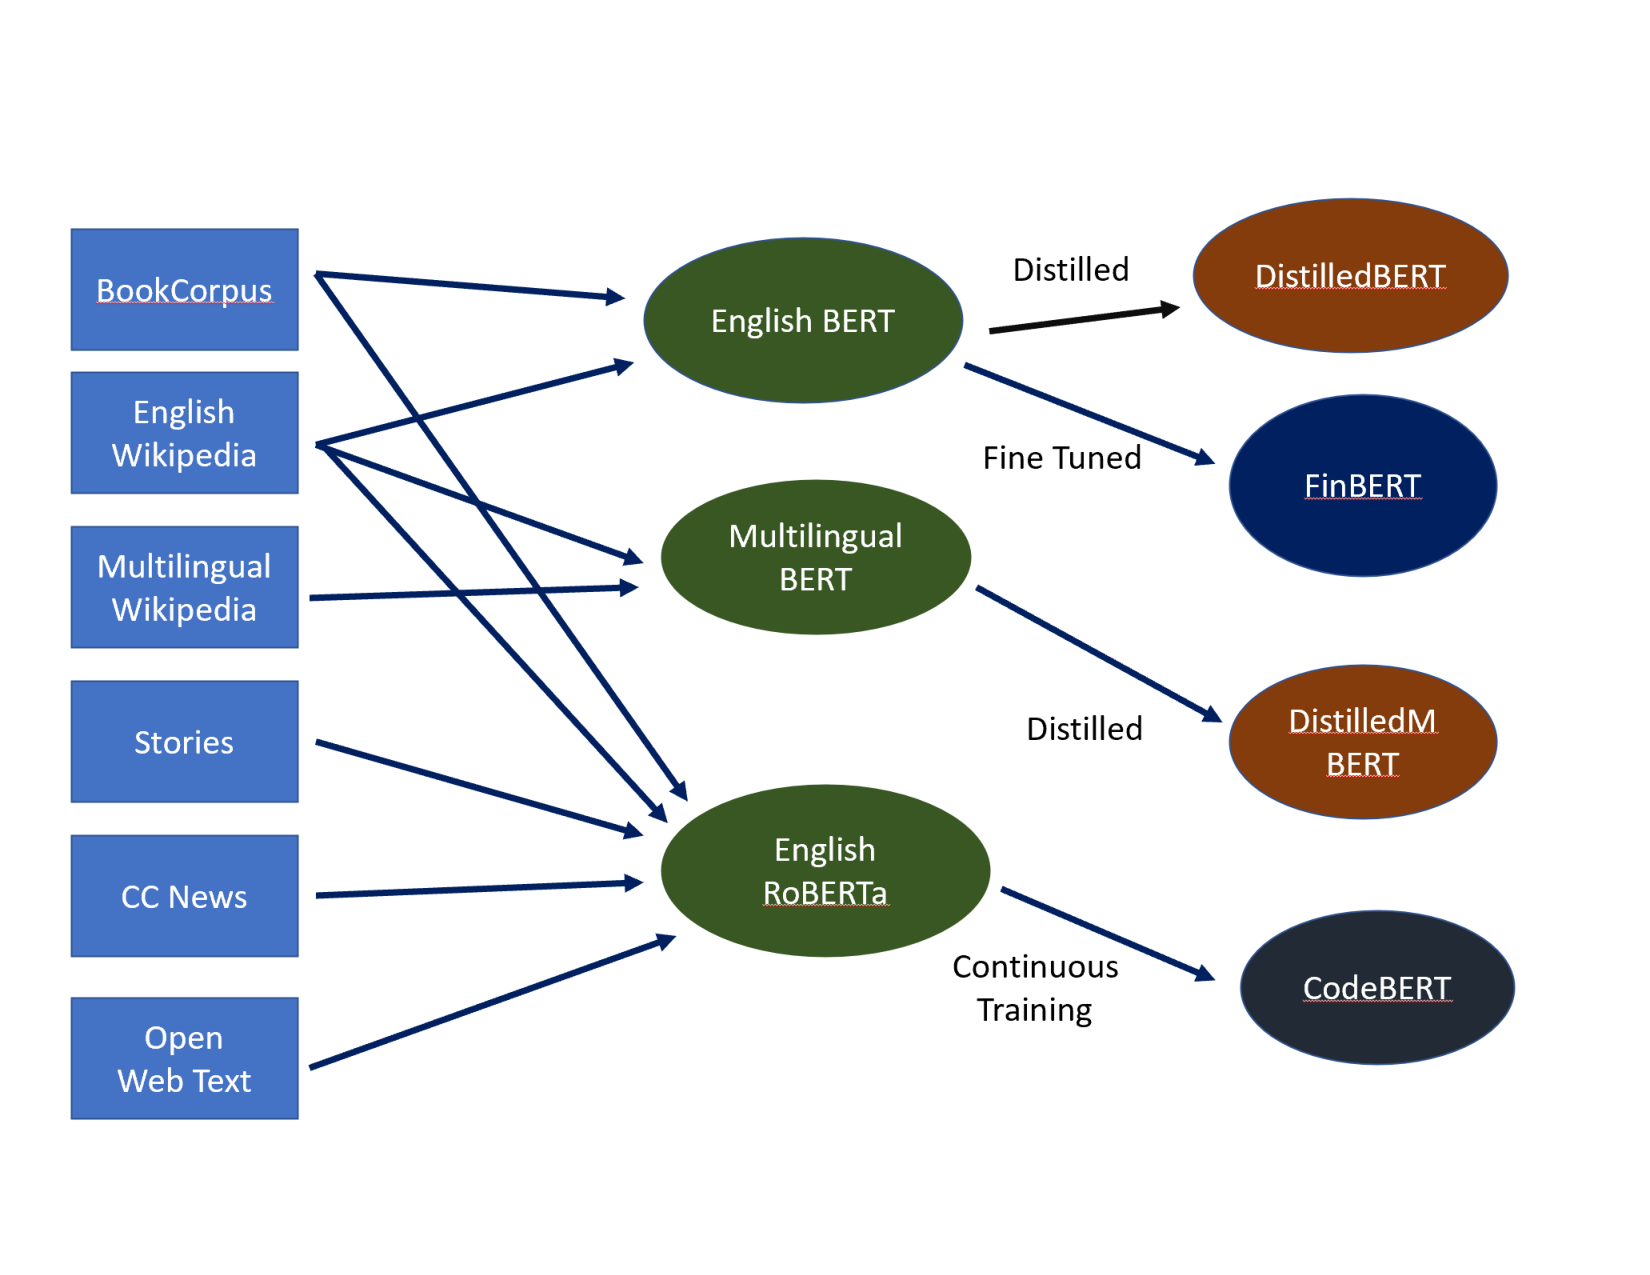
\includegraphics[width=8cm]{model-2.pdf}}
%%%\caption{The 'Supply Chain' of data-sets and models}
%%%  \label{fig:model-life-cycle}
%%%\end{figure*}
%
%\begin{figure}[]
%\centering{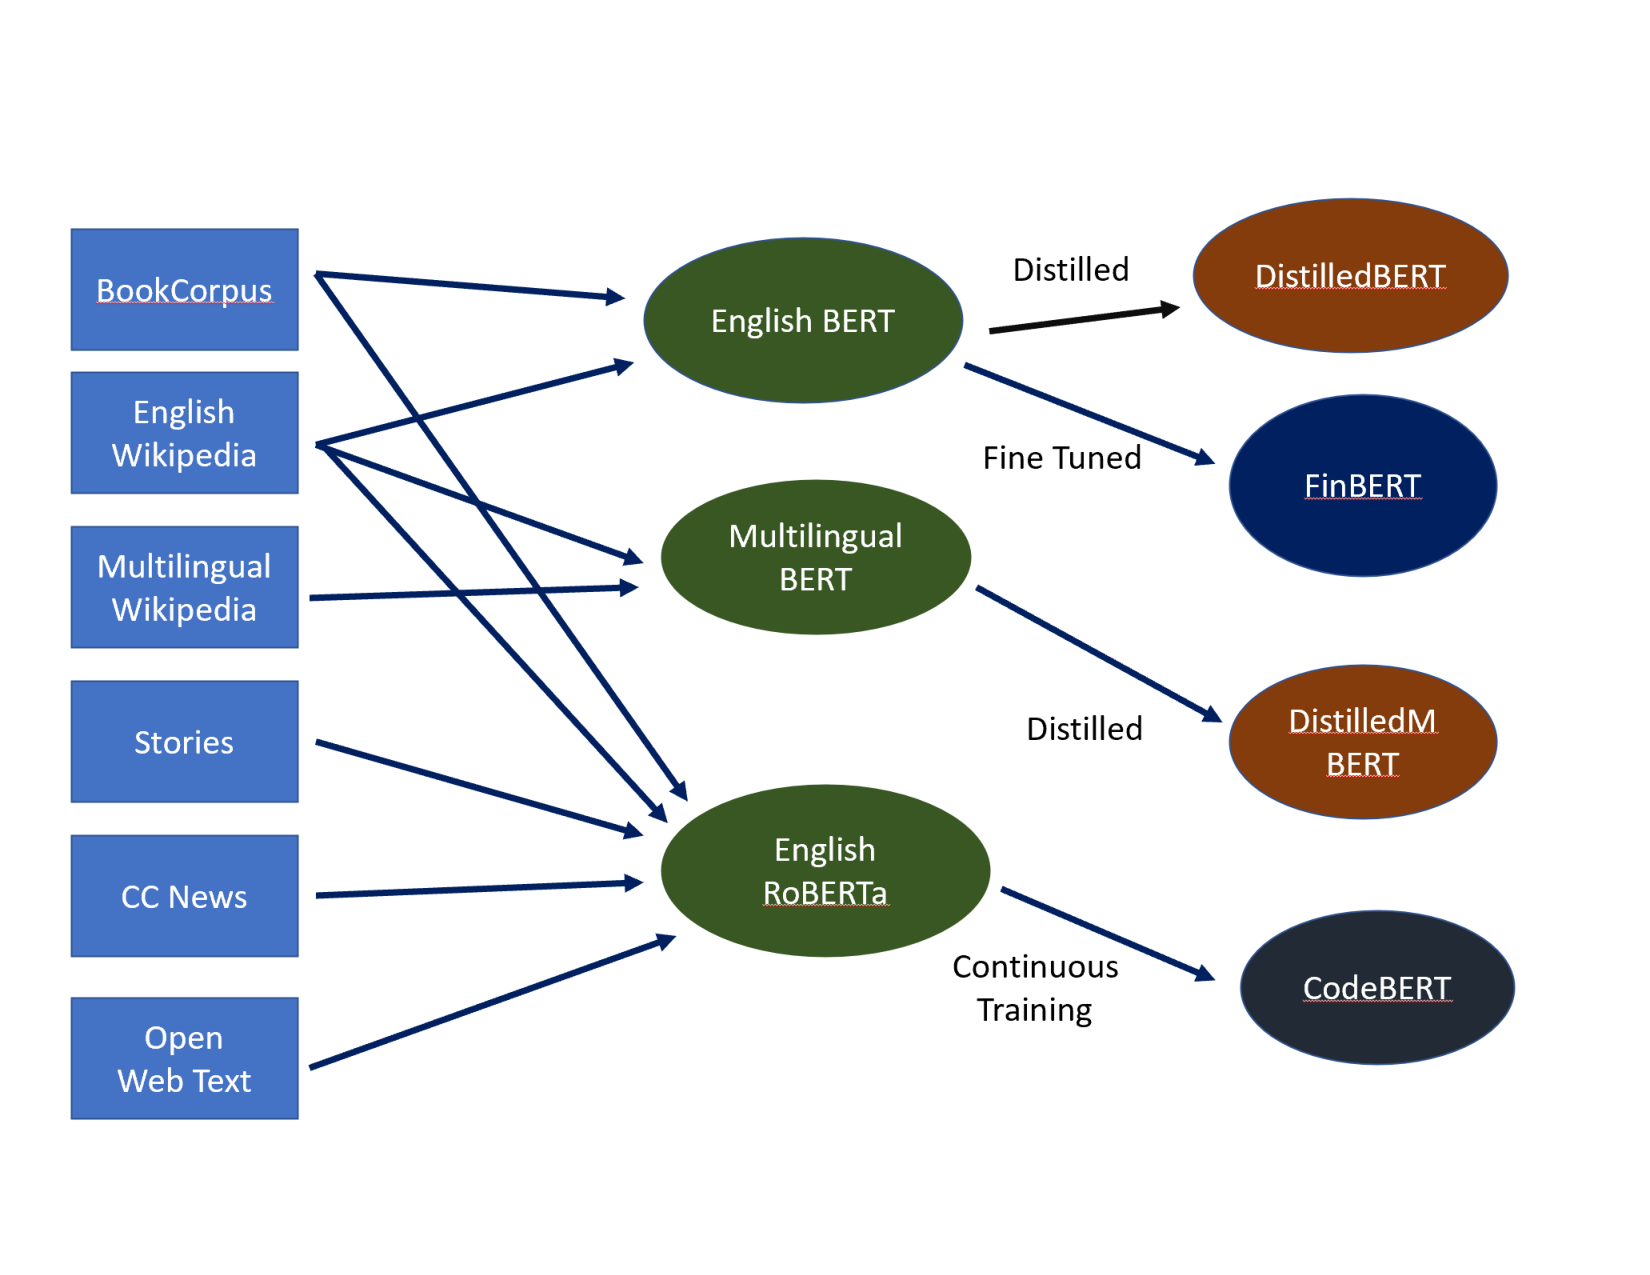
\includegraphics[width=8cm]{model-2.pdf}}
%\caption{The 'Supply Chain' of data-sets and models}
%  \label{fig:model-life-cycle}
%\end{figure}
%
%A pre-processing pipeline needed to curate data for training a model could consist of the following steps: Data acquisition:  Via crawling (for NLP) or running simulations (materials or physics); De-duplicating:  To ensure there Is one copy of a document from multiple sources; Selecting documents of certain languages of interest; Splitting the documents into sentences for training; Identifying Hate Abuse Profanity and PII information one may want to filter; Forming the data files for training based on a format
%For example, NLP datasets such as  Wikipedia,  Stories,  OpenWebText, BookCorpus, CC News which are constructed via web crawling. 
%Each of them could potentially be processed through all the above steps before it is ready for being used for training.  Fig \ref{fig:model-preprocess} shows such a pipeline
% 
% \begin{figure}[]
%\centering{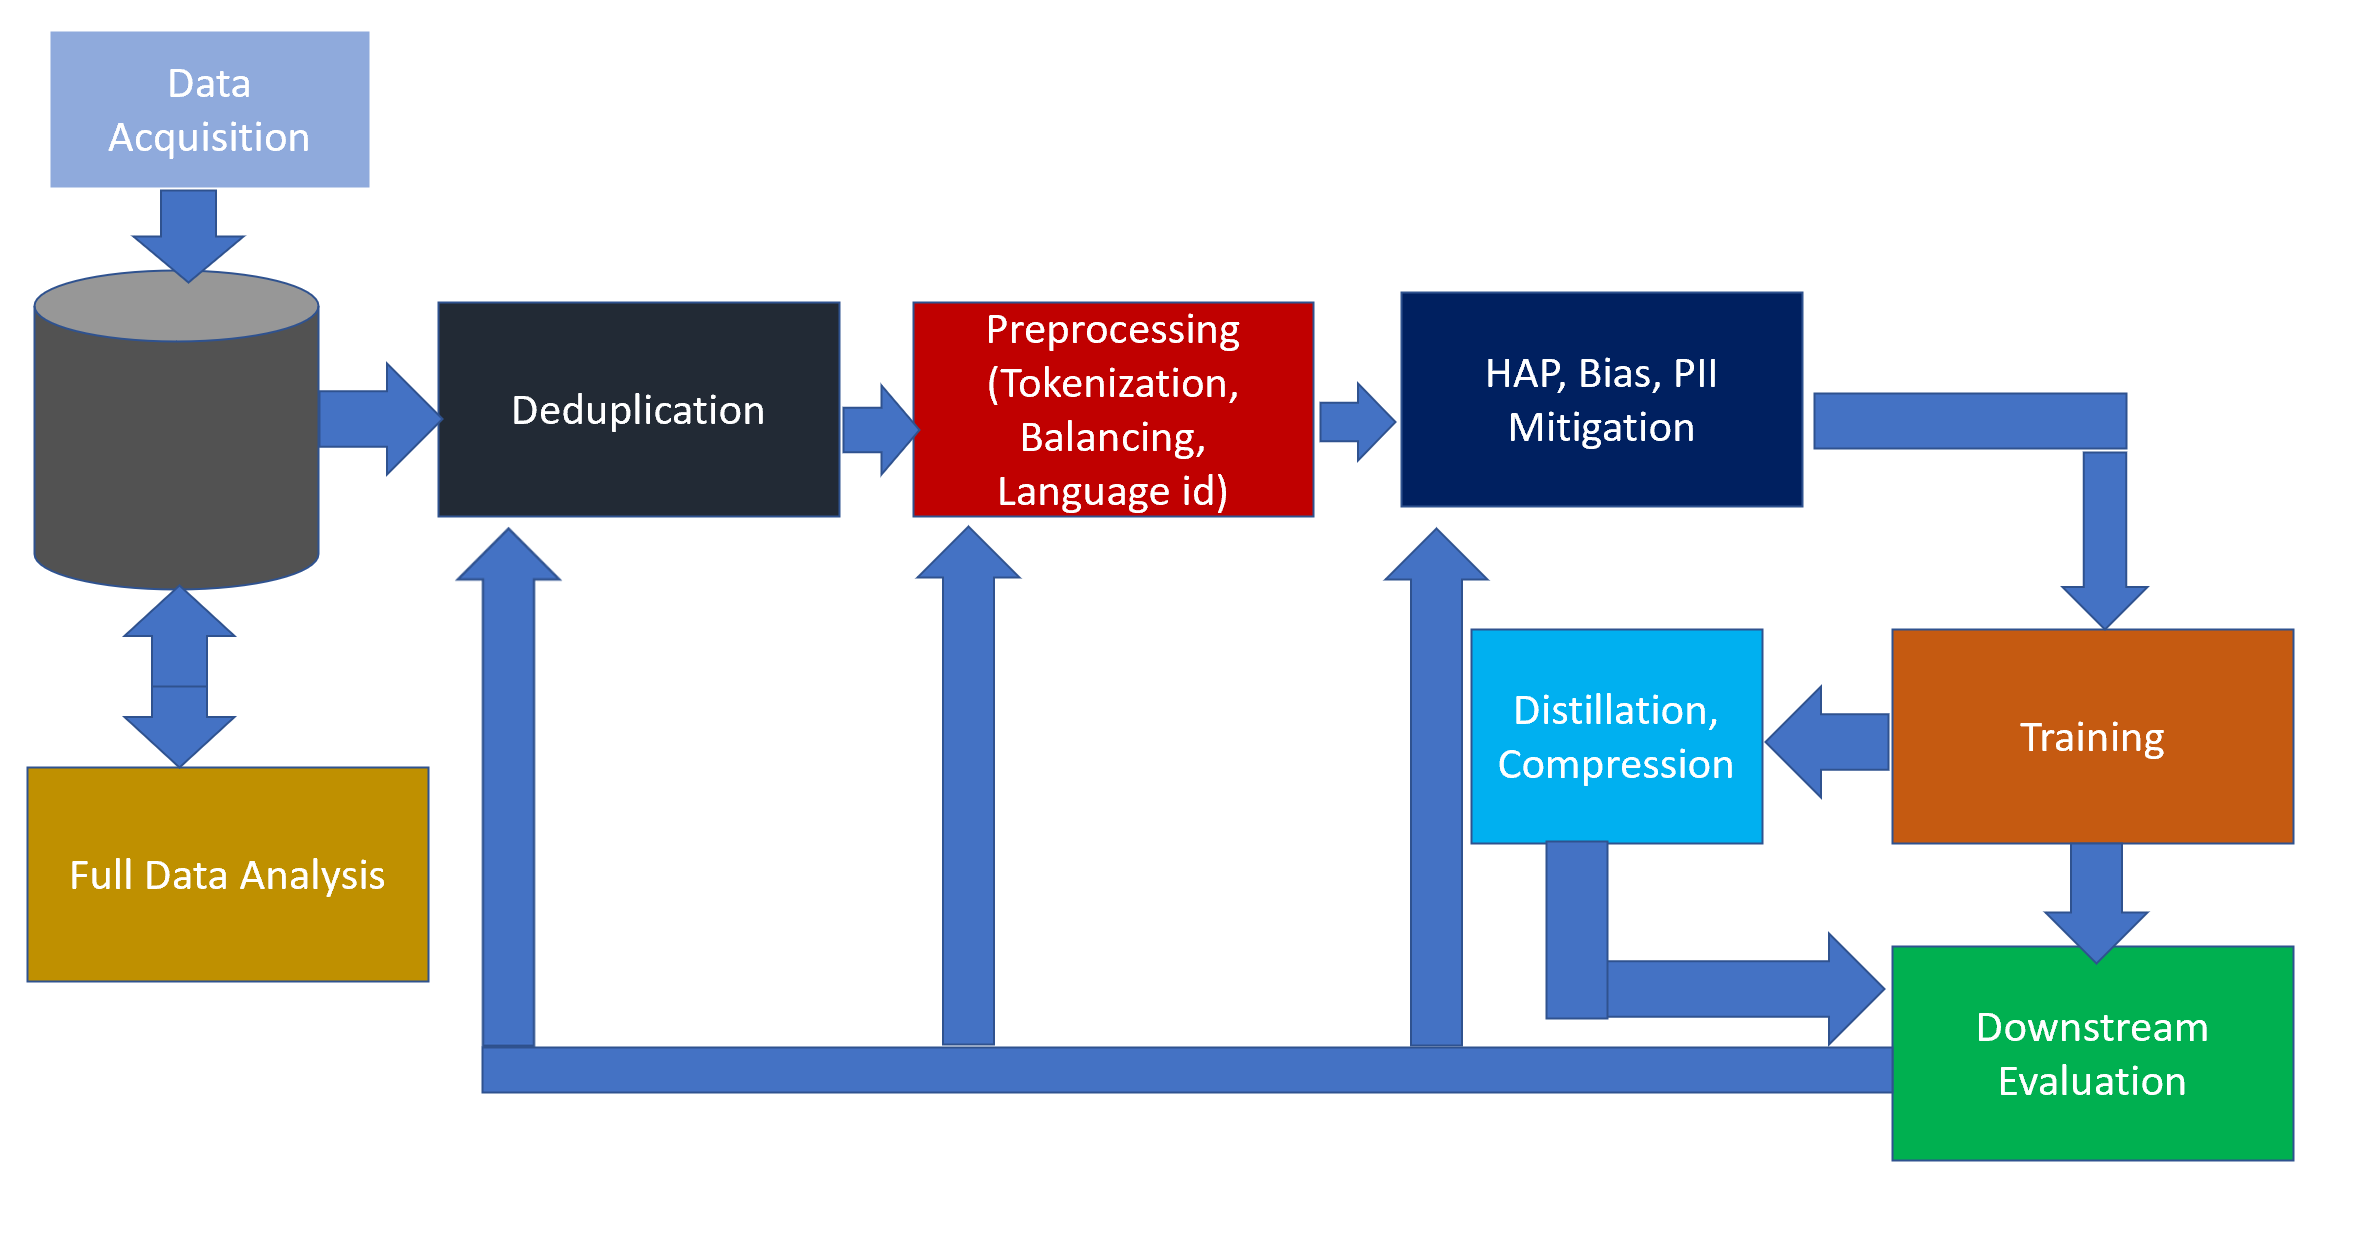
\includegraphics[width=8cm]{sustain3.png}}
%\caption{A typical preprocessing pipeline}
%  \label{fig:model-preprocess}
%\end{figure}
%
%
%These datasets have been used to train multiple models in various combinations.  BERT was trained using English Wikipedia and BookCorpus.  Whereas Multilingual BERT (mBERT) was trained on multilingual Wikipedia over 100+ languages.   RoBERTa on English data-sets spanning Wikipedia, Stories, OpenWebText, BoockCorpus as well as CC-News.  
%%The effort needed to curate this datasets gets amortized over multiple models which benefit from it in various proportions - will get to this later
%After a model is trained, the model may be distilled to bring it to a form factor which fits certain latency or space budget. For example  DistilBERT and DistilMBERT are based on BERT and mBERT respectively.  They are of 6 layers instead of the 12 layers in BERT and has $40\%$ less parameters then BERT base uncased; it runs $60\%$ faster while preserving $95\%$ pf the accuracy of BERT base on GLUE benchmark.
%
%The base model could also be further finetuned or  continuously trained for a certain domain. FinBERT was created by finetuning a BERT model on finance data and CodeBERT was created by continuously training RoBERTa over github repositories. FinBERT delivers better result than the base BERT on financial analysis benchmarks like FiQA Sentiment Scoring and Financial Phrasebank. There is some additional effort needed for fine-tuning and continuous training to produce these models.
%The effort needed to create the BERT base is now not only utilized when BERT is used directly on any task but also when models spun off from it are also utilized.

    \section{Towards Metrics and Methodology for Sustainable AI}
{
    \label{sec:metrics}

    As we stated above, our approach includes defining a new concept, which we term \textit{Embodied Product Cost} (Section~\ref{extensions}), then using it to expend the metric definition from~\cite{Gandhi2022} (Section~\ref{extensions}), and lastly, applying the result to the domain of AI (Section~\ref{application}).

    \subsection{Overview of Data Center Sustainability Metric}
    {
        \label{overview}

        In this section, we give a brief overview of two of the relevant metrics defined in~\cite{Gandhi2022}. The reader is referred to~\cite{Gandhi2022} for a complete description. All metrics defined, employ the unit of ``carbon dioxide equivalent" or gCO2e~\footnote{gCO2e stands for CO2 equivalent emissions, accounting for carbon dioxide and all the other greenhouse gases, such as methane and nitrous oxide}.

        The \textbf{Job Sustainability Cost (JSC)} is aimed at quantifying the carbon footprint associated with running a job. A \textit{job} is any unit of work, that an application performs relevant for scaling (i.e., work jobs require more resources). The Job Sustainability Cost (JSC) is calculated as the sum of energy used by the job's share of all systems participating in executing the job, and also including a `tax' for the cooling and power loss overheads. Energy is converted to carbon based on the mix of energy sources and their associated carbon. For example, consider a job $j$ that consumes $\unit[1]{kJ}$ energy executing on a host, and an additional $\unit[0.08]{kJ}$ due to cooling and power distribution losses. If the energy source mix is $80\%$ coal and $20\%$ solar, then, using carbon-intensity values (and converting kJ to kWh), we have $JSC \! \left ( j \right ) = 1.08 \times (0.8 \times 820 + 0.2 \times 48) \div 3600 \approx \unit[0.2]{gCO2e}$.  

        The \textbf{Amortized Sustainability Costs (ASC)} is aimed at further including an additional `tax' for the life cycle cost of the systems used in the computation. It is calculated by adding the job’s share (or tax) of the systems' embodied emission and other costs of all systems participating in the computation to the previously defined $JSC$. For the job $j$ from the example above, assume that it runs exclusively for $5$ minutes on a system $S$ with an expected lifetime of $3$ years, and the embodied cost of $S$  is $\unit[10,\!000]{gCO2e}$. Let $ec \! \left ( j \right )$ be the `tax' for embodied carbon. Then, $ec \! \left ( j \right ) = 10,\!000 \times \frac{5}{3\times 365 \times 24 \times 60} = 0.031$, and $ASC \! \left ( j \right ) = JSC \! \left ( j \right ) + ec \! \left ( j \right ) \approx \unit[0.231]{gCO2e}$. 

        The paper defines other useful metrics, such as {\bf Job Quality per Cost Rate (JQCR)} which we will not get into here due to space limits. 
    }

    \subsection{Proposed Extension}
    {
        \label{extensions}

        We agree with \cite{Gandhi2022} that an end-to-end data center sustainability metrics must ultimately focus on the cost of a unit of work executed, and that all overheads to the extent possible, must be added in. However, one overhead which is not accounted for in the definitions in Section~\ref{overview}, is that of a job \textit{execution context}. Most jobs today, in cloud or on-premise environments, execute in a context of a continuously running shared software platform. For example, a Serverless job on AWS executes in the context of a platform termed Lambda~\cite{Lambda}. A container in IBM Cloud, is executed in a context of a platform termed IBM Kubernetes Service (IKS)~\cite{IKS}. There are significant overheads associated with the operations and life cycle of these platforms. For example, in IKS, there are a number of servers dedicated to managing the service in every location where the service is deployed. These management servers are always running, independently of the number of jobs executing. They are used to run management software to, e.g., monitor the health of the systems, and to meter usage for billing purposes. In storage and data services, such as IBM's Cloud Object Storage (COS) ~\cite{COS}, processes wake up periodically, unprompted by any user initiated action, to perform cleanup, and tier management. Other shared services may be used across services (i.e., logging service), and the proportionate share of their use must be taken into account as well (see, ~\cite{Eilam2021}). In addition, we ought to not forget about the cost of continuous deployment (CD), and testing of the platform. 

        We use the term \textit{software product} (in short, \textit{product}) to denote any software asset, such as, a software platform that is used as-a-services to support the execution of jobs, or, an AI model used in serving inference requests, or, a datasets which are prepared and then used for the training of AI models, etc. Each software product is associated with a life cycle, including development, deployment, and use. 

        Next, we define a new metric to capture the `embodied' carbon of software products, according to the same principles that are used for calculating the embodied carbon of systems. For systems, activities include material extraction, transportation, manufacturing processes, etc, factoring-in the \textit{em entire supply chain} leading to the end product. For software, activities may vary based on the type of software product. For a platform delivered as a service they will include development and testing; for a dataset it includes data preparation and de-duplication; and, for an AI model it includes training. Each such activity consists of humans working on systems that consume energy from certain power grid, with a particular energy mix. 

        The \textbf{Embodied Product Cost (EPC)} is the upfront development cost of any given software product (up to the point of its deployment and use). It is calculated as the carbon footprint associated with all activities needed to create the product. We can for example refer to an activity of a developer, or, a tester, or a data scientist, a day, as a job $j$. The Embodied Product Cost $EPC$, is the summation over all $ASC \! \left ( j \right )$ of all the jobs over the course of the creation of the product (a period that can easily take a couple of years).  

        Next, we propose to expand the definition of $JSC$ to factor-in the platform's operational cost. To avoid confusion, we denote the expanded definition as $JSC^e$.

        The \textbf{Expanded Job Sustainability Cost} (denoted $JSC^e$) is calculated as the sum of energy (converted to carbon) of all systems participating in the computation, and a `tax' for cooling and power loses, and a `tax' for the platform overhead if a platform is used as the execution context. For example, assume that the job $j$ is a container that runs in the context of a platform such as IBM's IKS~\cite{IKS}. This platform, in a particular location such as Dallas, uses $3$ servers dedicated to management, and their associated carbon is $\unit[50]{gCO2e}$ for every minute of operation. Let's assume that the job $j$ executes for $5$ minutes, and that while it is executing, there are concurrently $9$ other jobs, of roughly equal size, executing on IKS in Dallas. Then, our job is `taxed' $\frac{50}{10} \times 5$ for its share of the platform overhead. This number is added to $JSC \! \left ( j \right )$ to derive $JSC^e \! \left ( j \right )$.  In addition, we also need to add the cost of service maintenance, and continuous development and testing. We leave this as an exercise to the reader. 

        Lastly, we expand accordingly the definition of the Amortized Sustainability Cost ($ASC$) of jobs. We claim that in addition to the embodied emission of systems participating in the execution of a job, we also have to add the embodied emission of any software product that serves in the execution.

        The \textbf{Expanded Amortized Sustainability Cost}, denoted, $ASC^{e}$, is calculated as the sum of $JSC^{e}$, and, the job’s share (or tax) of the systems' embodied emission (for all systems participating in the computation), and, the Embodied Product Cost (EPC) of the platform supporting the computation. As an example, if $j$ is a container running on IKS, in Dallas, and it runs for $5$ days, concurrently with $9$ other equally sized jobs, and lets us assume that the expected life time of the IKS service in Dallas is $6$ years, then it is taxed $EPC \! \left ( IKS \right ) \times \frac{5}{10 \times 365 \times 6}$, which is added to $ASC \! \left ( j \right )$ to derive $ASC^{e} \! \left ( j \right )$. 

        With the introduction of a new metric $EPC$ to capture the embodied cost of software products, and with the expanded definition of $JCS$ and $ASC$, we are now ready to turn our attention to the unique and fascinating life of AI models. We show how we apply these three metrics to meaningfully calculate the sustainability cost of AI inference jobs. 
    }

    \subsection{Metrics for Sustainable AI} 
    {
        \label{application}

        We are now ready to apply the concepts and definitions from Section~\ref{extensions} towards metrics for Sustainable AI. 

        There are two `products' that are of key relevance for AI. The first is a dataset. Refer to Section~\ref{life-cycle} for activities used to create a dataset. Once a dataset is ready, it can be used to train multiple different models. For a dataset $d$, we calculate the Embodied Product Cost $EPC \! \left ( d \right )$ as the sum of carbon footprint of all activities involved in preparing the dataset. If we refer to each such activity as a single job then $EPC \! \left ( d \right ) = \sum_{j} ASC^{e} \! \left ( j \right )$. 

        The second `product' that is relevant to AI, is an AI model. A model is prepared (i.e., developed, or `manufactured') via a process of experimentation, and training (see Section~\ref{life-cycle}) leveraging one or more datasets. A given model can also be used to develop another, sometimes task-specific, model, in a process called \textit{distillation} or \textit{fine-tuning}. 

        For a model $m$, $EPC \! \left ( m \right )$ is calculated as the sum of the carbon footprint associated with the development (`manufacturing') of a model, recursively. Formally, $EPC \! \left ( m \right ) = ASC^{e} \! \left ( j \right ) + w_{1} \times EPC \! \left ( m^{\prime} \right ) + w_2 \times \sum EPC \! \left ( d_{i} \right )$, where, $j$ is defined as the `job' of preparing $m$ based on either another model $m^{\prime}$ or multiple datasets $d_{1}, d_{2}, \dots$ and,  $w_{1}$ is a tax weight to factor-in the re-use of a different model $m^{\prime}$. It is $0$ if there was no model that was re-used, or proportioned, based on its share of model re-use, and finally, $w_{2}$ is the tax weight, if the model was created based on datasets $d_{1}, d_{2}, \dots$. It is $0$ if there was no dataset that was used, or proportioned, based on its share of re-use. As an example, consider the RoBERTa model (\cite{Liu2019}). It was pre-trained based on a set of datasets (Wikipedia, CC-NEWS, Stories, OpenWebText, BookCorpus), using $1024$ $\unit[32]{GB}$ NVIDIA V100 GPUs for approximately one day. Assuming that the GPUs were working at full capacity, the maximum power consumption is $\unitfrac[300]{J}{s}$. Thus, the energy consumed for pre-training is $1024 \times 300 \times 360 \times 24 = \unit[737]{kwh}$. We still have to add cooling/power-loss overheads, as well as, the `tax' for the embodied system carbon footprint of the GPUs, as well as the fraction of embodied product carbon of the datasets used $EPC \! \left ( \text{CC} - \text{NEWS} + \text{BookCorpus} + \text{Wikipedia} + \text{OpenWebText} + \text{Stories} \right )$ (and then convert to carbon based on the grid energy mix). Yet as another example, DistilBERT (\cite{Sanh2019}), was created based on BERT via distillation. It has about half the total number of parameters of BERT base and retains $95\%$ of BERT’s performances on the language understanding benchmark GLUE. To create DistilBERT based on BERT, the team (\cite{Sanh2019}) used eight \unit[16]{GB} V100 GPUs for approximately three and a half days. Again assuming GPUs were used to their max capacity ($\unitfrac[250]{J}{s}$) the energy for distillation turns out to be $\unit[14.4]{kWh}$, and we need to add a tax for the fraction of re-use of BERT based on its $EPC$, and the other components as explained above.

        Once a model is `ready' it is deployed, and used to serve inference jobs. We can say that a model is \textit{deployed} when it is available to be used to serve inference jobs. We can refer to the life cycle phase when it is serving inference jobs as \textit{the operational phase}.
        
        In addition  to serving inference jobs, the model must be kept accurate, thus, it is being continuously re-trained. The frequency of re-training, and the cost of it, varies across models, and use cases. For example, in~\cite{Wu2022}, the frequency reported for two different use-cases is daily, and weekly. 

        Let's assume that at time interval $t$, a model $m$ was used to serve $n$ inference jobs, and the carbon cost of re-training at that interval was $cf_{rt}$ (note, there may have been multiple re-training `jobs' at time interval $T$, in which case we take their sum). Then, the carbon cost of re-training $cf_{rt}$, must be split equally (or in proportion to the size, for non-equal jobs), across all jobs executing at time interval $t$, i.e., $cf_{rt} / n$ is added.

        As an example, inference jobs based on DistilBERT take $\approx 410$ seconds to complete on CPU (Intel Xeon E5-2690 v3 Haswell @2.9GHz), which translate to $\approx \unit[0.015]{kWh}$ of energy. This is about $60\%$ of the cost of inference with the original BERT. This demonstrates the benefits of tolerating the additional upfront cost associated with  distillation, for downstream efficiency gains. To calculate $JCA^{e}$ we need to also include the cost of re-training which is use case specific. Adding in the cost of model re-training will encourage data scientists to practice sustainability mindset, examining, for example, the needed frequency.

        Finally, lets now discuss how we calculate $ASC^{e} \! \left ( j \right )$, where $j$ is an inference job performed against a model $m$. Here, we leverage our Embodied Product Cost metric ($EPC \! \left ( m \right )$), in order to account for the carbon associated with  the construction of a model, as well as the embodied system cost. Thus, $ASC^{e} \! \left ( j \right )$ is calculated adding in both. For a model $m$, if the lifetime expectancy of the model is $LT$, for example, $3$ years, and the execution time of an inference job is $t$, and there are $n$ parallel jobs executing at any given time, then $ASC^{e} \! \left ( j \right ) = ASC \! \left ( j \right ) + \frac{EPC \! \left ( m \right ) \times t}{LT \times n}$, where $ASC \! \left ( j \right )$ is defined as expected, adding to $JSC^{e} \! \left ( j \right )$ the embodied system emission tax, and related costs. 

        Again, this metric exemplifies the usefulness for fostering a sustainability mindset. A datasetentist will be encouraged to ask questions, such as `what is the right allocation of energy to train a model based on the expected usage, and expected life time'. 
    }
}

    \section{Opportunities}
{
    \label{opportunities}

    A fundamental requirement would be to establish a reliable system to collect, store and report data concerning the power/energy utilization across the complete lifecycle of the AI model. Such a challenge poses significant difficulties as certain facilities may lack the capacity for monitoring or measuring. Furthermore, even in facilities equipped with monitoring capabilities, the methodologies employed for measuring power/energy could vary widely, such as how to allocate shared resources for model training. Consequently, this issue can be bifurcated into two principal aspects: standardization and reliable information tracking.

    First and foremost, it is important to standardize the procedures employed for measuring, collecting, and reporting {power/energy/} carbon consumption data pertaining to the AI model. This measure would enable consistent and comparable reporting metrics. This paper takes a step towards that goal, more work is needed on the system energy consumption, in particular in lieu of sharing. Additionally, it is important to ensure accuracy and integrity of the records. 
Models and data sets should be published with a data sheet that reports based on the metrics. Yet another area is use case based optimization. The first advantage of the proposed approach is mind-set shifts in the AI model design process. Historically, AI models have been developed with an emphasis on performance. However, upon considering our AI lifetime observability matrics, system designers would begin to prioritize both performance and energy efficiency in their AI model architectures, as evidenced by factors such as neural network depth, width, input resolution, and parameters~\cite{Desislavov2023}. This would facilitate the development of AI models that are not only high-performing but also energy-efficient, thereby reducing the need for unnecessary training practices. In particular, it would be necessary to develop methods to compare different life cycle strategies in the context of use cases, i.e., re-use (and what) vs. start from scratch. 

    Furthermore, this approach would allow for the identification of inefficiencies within the various phases of AI, which could be targeted for optimization. Through the implementation of scheduling techniques and power knob configurations (such as power capping and dynamic voltage and frequency scaling), we would be able to enhance the utilization of each resource while simultaneously reducing energy consumption. 
}

    
    \appendix

    % Bibliography
    \bibliographystyle{ACM-Reference-Format}
    \bibliography{references}
\end{document}

